\chapter{Scenario Series 6-1}

This document presents simulation results from the scenario series 6-1, which tests impact of varying planning horizon length for both principal and agent. 
We test all combinations of horizon lengths for values 30, 20, 10, 5,  and 1 (periods). 
Note that agent horizon is never allowed to be longer than principal horizon.

\section{Summary}
Table \ref{tab:scenario_list} below lists the scenarios in series 6-1. 
Control scenario s6-0 simulates the \emph{status quo} situation (single-level wood supply model with no anticipation of fibre consumption).  

\begin{table}
  \centering
  \begin{tabular}{lll}
    \hline
    Scenario ID & Figure Reference & Description \\
    \hline
    6-0 & \ref{fig:s6-0} & Control scenario. \\
    6-1\_p30a30 & \ref{fig:s6-1_p30a30} & Principal: 30 periods, agent: 30 periods. \\
    6-1\_p30a20 & \ref{fig:s6-1_p30a20} & Principal: 30 periods, agent: 20 periods. \\
    6-1\_p30a10 & \ref{fig:s6-1_p30a10} & Principal: 30 periods, agent: 10 periods. \\
    6-1\_p30a05 & \ref{fig:s6-1_p30a05} & Principal: 30 periods, agent: 5 periods.   \\
    6-1\_p30a01 & \ref{fig:s6-1_p30a01} & Principal: 30 periods, agent: 1 period.     \\
    6-1\_p20a20 & \ref{fig:s6-1_p20a20} & Principal: 20 periods, agent: 20 periods.\\
    6-1\_p20a10 & \ref{fig:s6-1_p20a10} & Principal: 20 periods, agent: 10 periods.\\
    6-1\_p20a05 & \ref{fig:s6-1_p20a05} & Principal: 20 periods, agent: 5 periods. \\
    6-1\_p20a01 & \ref{fig:s6-1_p20a01} & Principal: 20 periods, agent: 1 period.  \\
    6-1\_p10a10 & \ref{fig:s6-1_p10a10} & Principal: 10 periods, agent: 10 periods.\\
    6-1\_p10a05 & \ref{fig:s6-1_p10a05} & Principal: 10 periods, agent: 5 periods. \\
    6-1\_p10a01 & \ref{fig:s6-1_p10a01} & Principal: 10 periods, agent: 1 period.  \\
    6-1\_p05a05 & \ref{fig:s6-1_p05a05} & Principal: 5 periods, agent: 5 periods. \\
    6-1\_p05a01 & \ref{fig:s6-1_p05a01} & Principal: 5 periods, agent: 1 period.  \\
    6-1\_p01a01 & \ref{fig:s6-1_p01a01} & Principal: 1 period, agent: 1 period.  \\
    \hline
  \end{tabular}
  \caption{Description of scenarios in series 6-4.}
  \label{tab:scenario_list}
\end{table}

\section{Results}

Figures \ref{fig:s6-1p30a30} to \ref{fig:s6-1p01a01} present
simulation results for fifteen scenarios. % Table \ref{tab:scenarios}
% summarizes scenario parameters used in the experiment for each
% scenario.
Disposition of figures is identical for all scenarios. The
first subfigure (a) for each scenario shows the initial
(ie. iteration-0) AAC solution. The second subfigure (b) for each
scenario shows first period of AAC solution for all 30 planning
iterations. The third subfigure (c) for each scenario shows the
implemented harvest level for all 30 planning iterations. Scenarios
3.1 and 3.2 also show profit in this subfigure on a secondary
axis. The fourth subfigure (d) for each scenario shows the difference
between initial and re-planned AAC. The fifth subfigure (e) for each
scenario shows the difference between re-planned AAC and harvest.  The
sixth subfigure (f) for each scenario shows the difference between
initial AAC and harvest. Softwood volume is shown with white bars,
hardwood volume with black bars, and total volume with small
circles. Profit (where applicable) is shown with the $\times$
symbol. 

\begin{figure}[h]
  \centering
  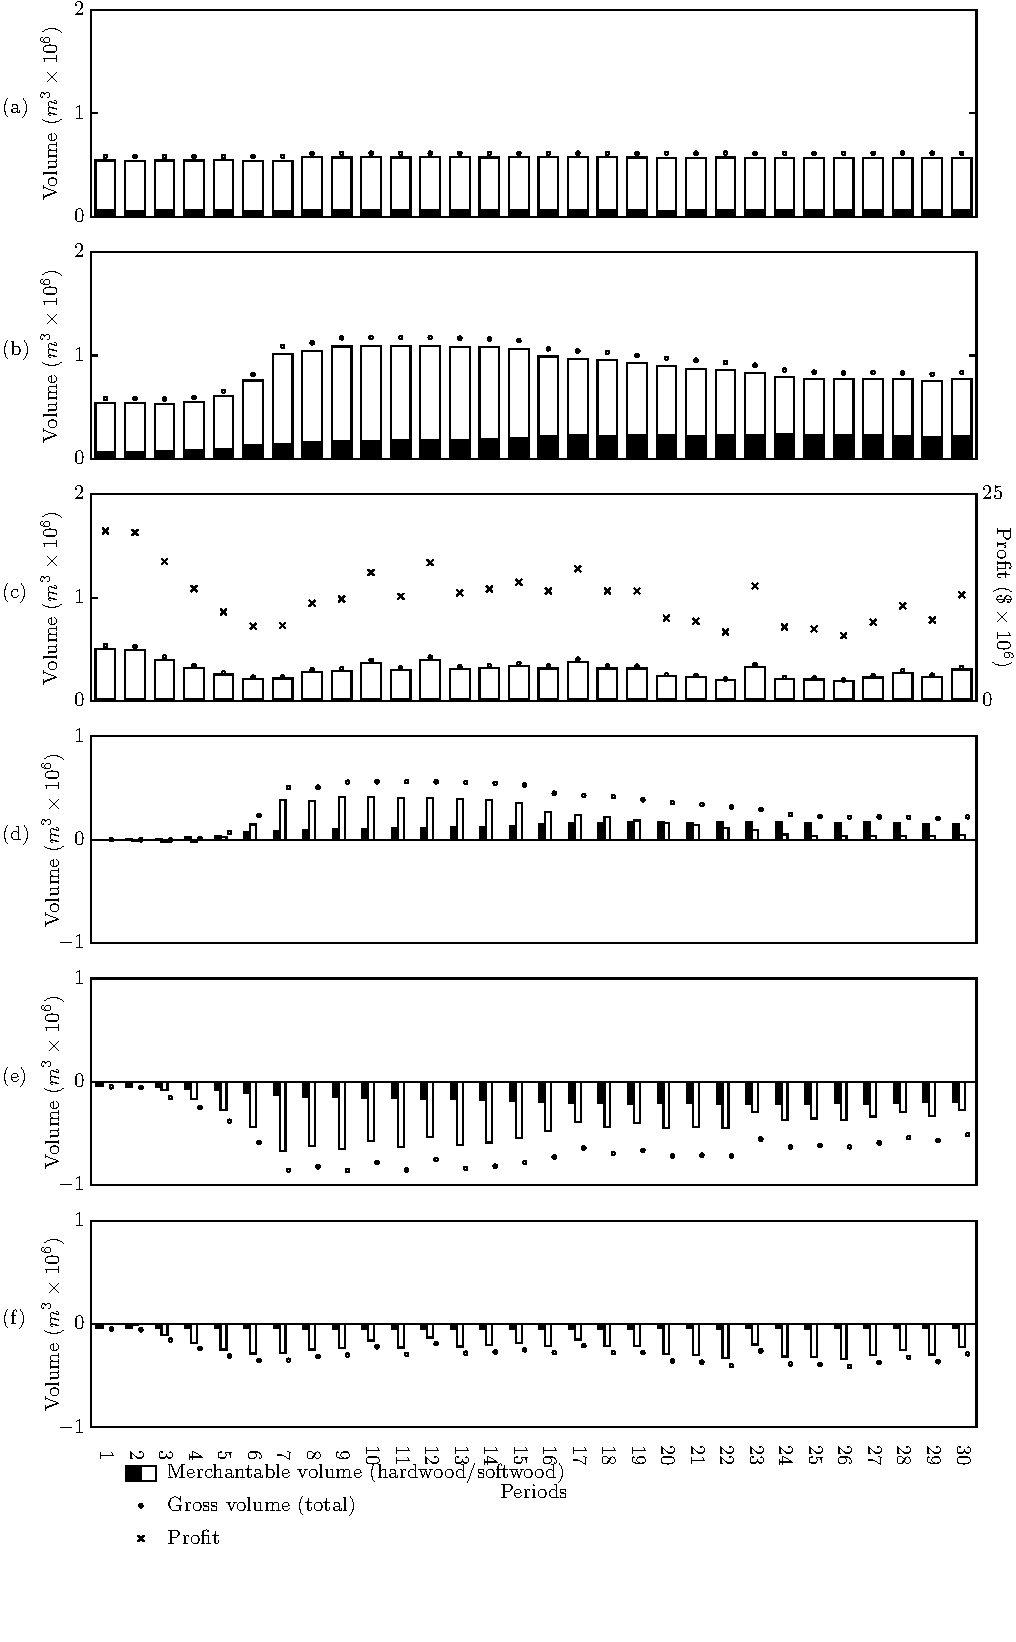
\includegraphics[width=10cm]{images/appendix/s6-0}
  \caption{Scenario 6-0 (control scenario, simulates \emph{status quo}).}
  \label{fig:s6-0}
\end{figure}


\begin{figure}[h]
  \centering
  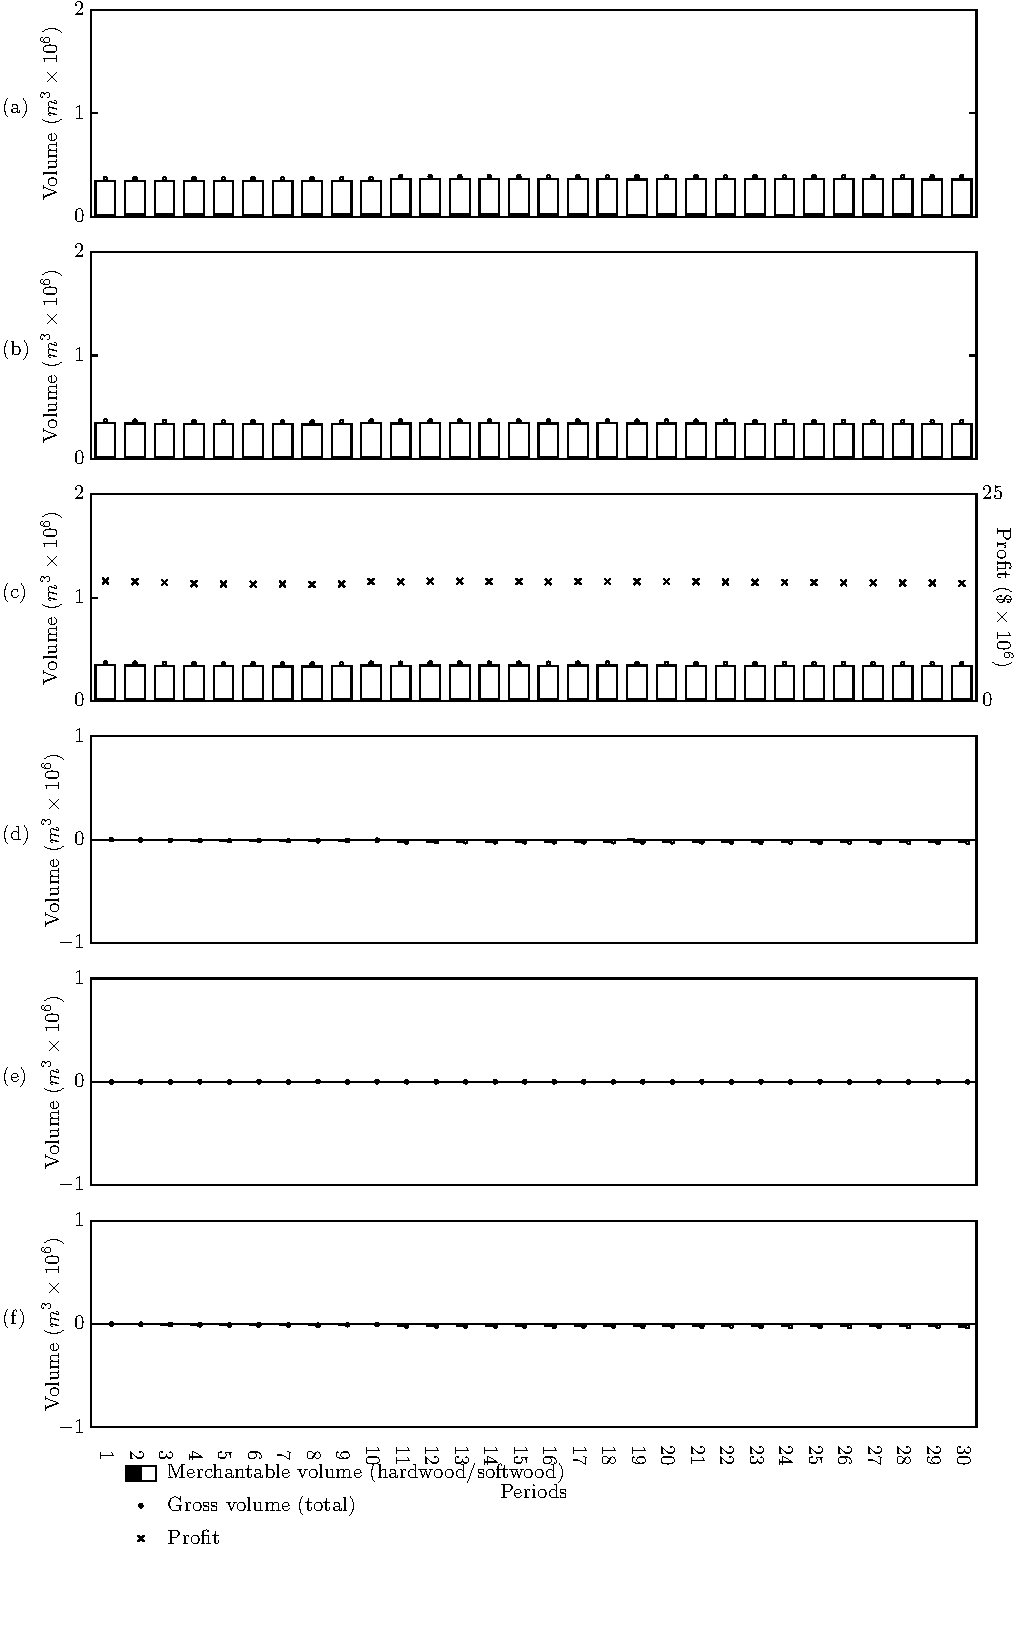
\includegraphics[width=10cm]{images/appendix/s6-1_p30a30}
  \caption{Scenario 6-1\_p30a30 (principal: 30 periods, agent: 30 periods).}
  \label{fig:s6-1_p30a30}
\end{figure}

\begin{figure}[h]
  \centering
  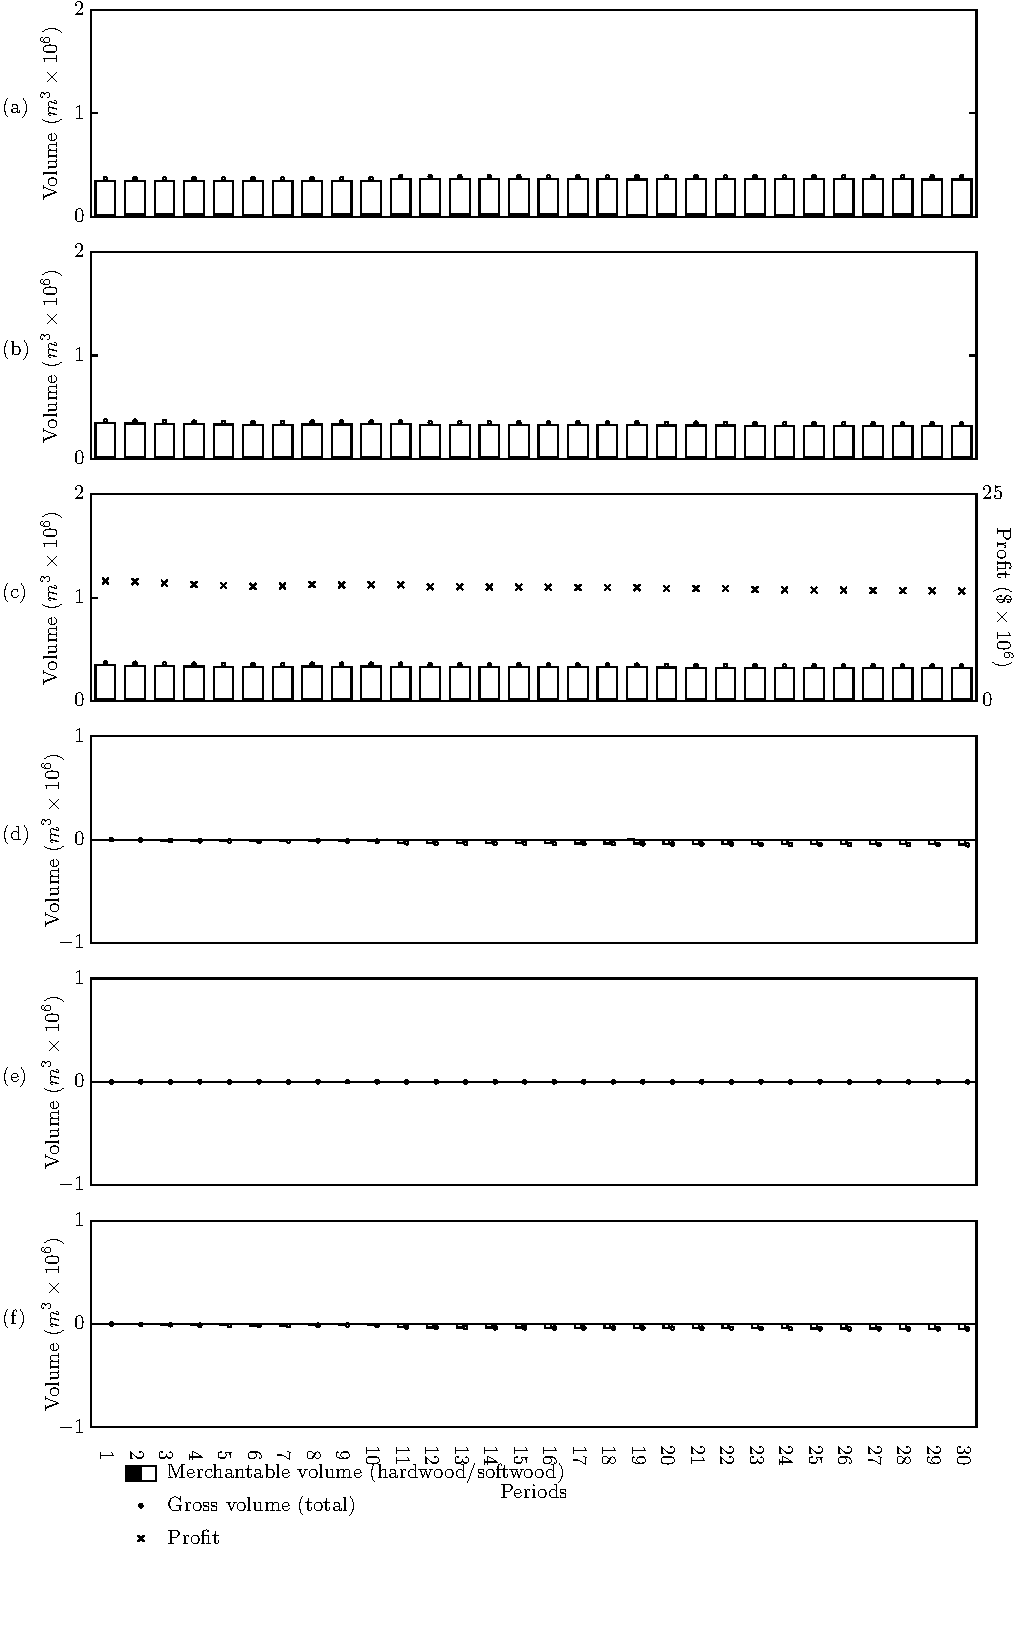
\includegraphics[width=10cm]{images/appendix/s6-1_p30a20}
  \caption{Scenario 6-1\_p30a20 (principal: 30 periods, agent: 20 periods).}
  \label{fig:s6-1_p30a20}
\end{figure}

\begin{figure}[h]
  \centering
  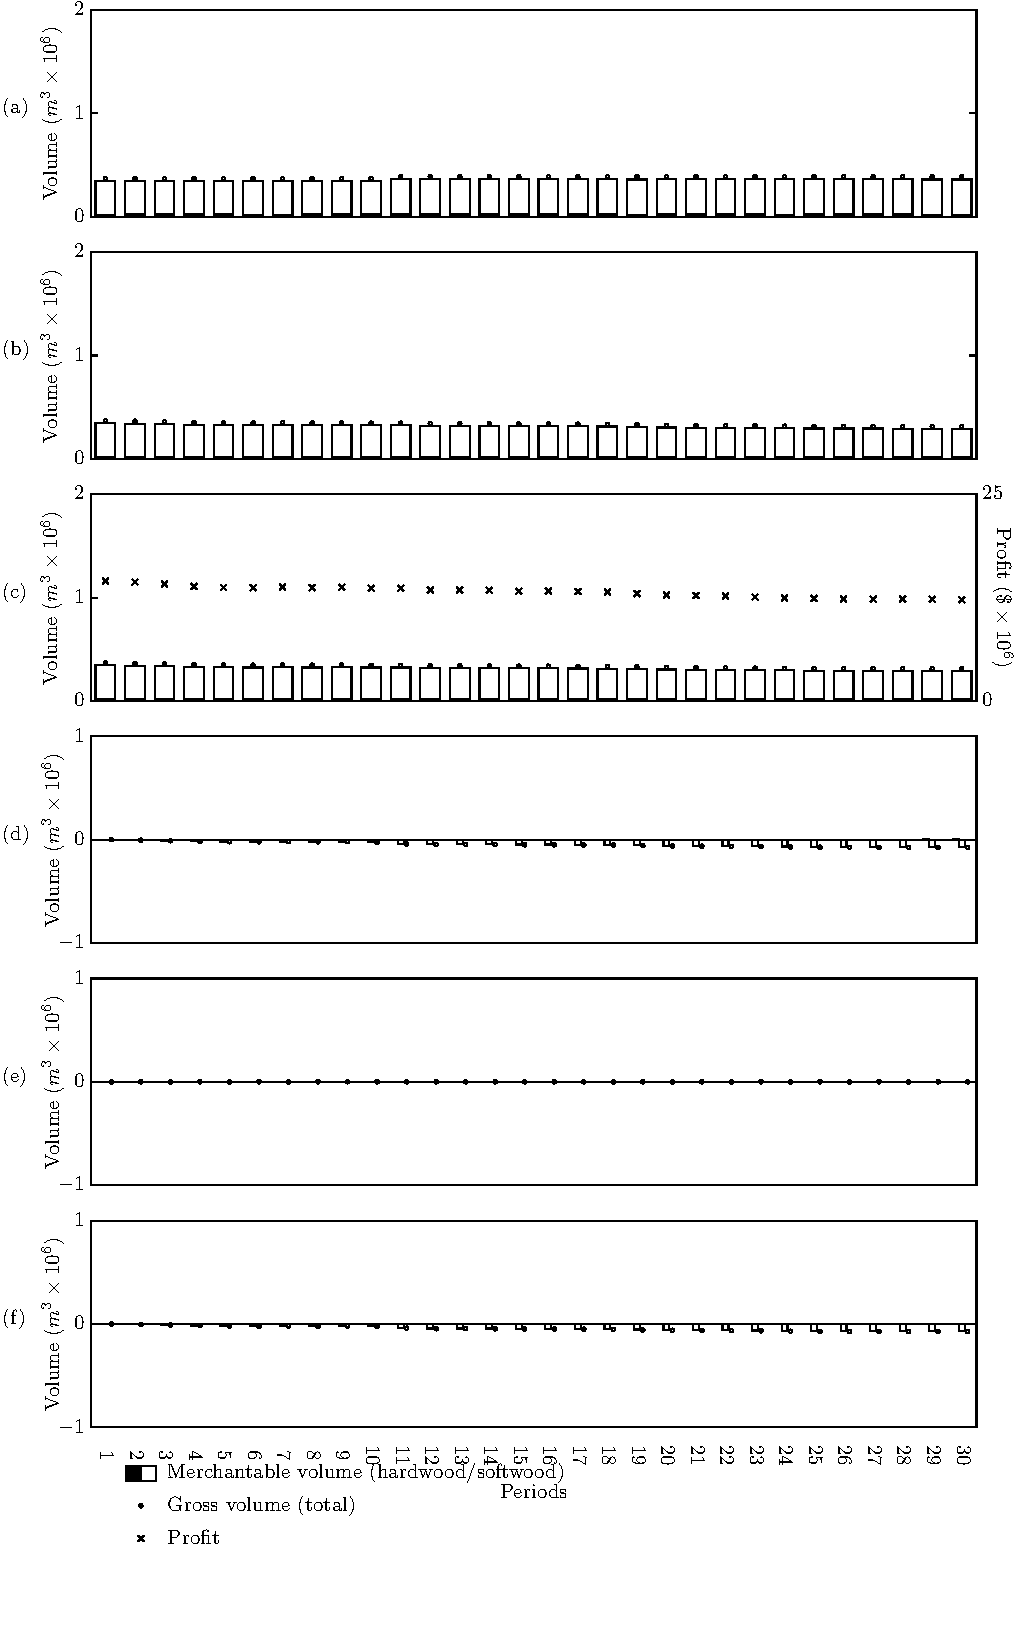
\includegraphics[width=10cm]{images/appendix/s6-1_p30a10}
  \caption{Scenario 6-1\_p30a10 (principal: 30 periods, agent: 10 periods).}
  \label{fig:s6-1_p30a10}
\end{figure}

\begin{figure}[h]
  \centering
  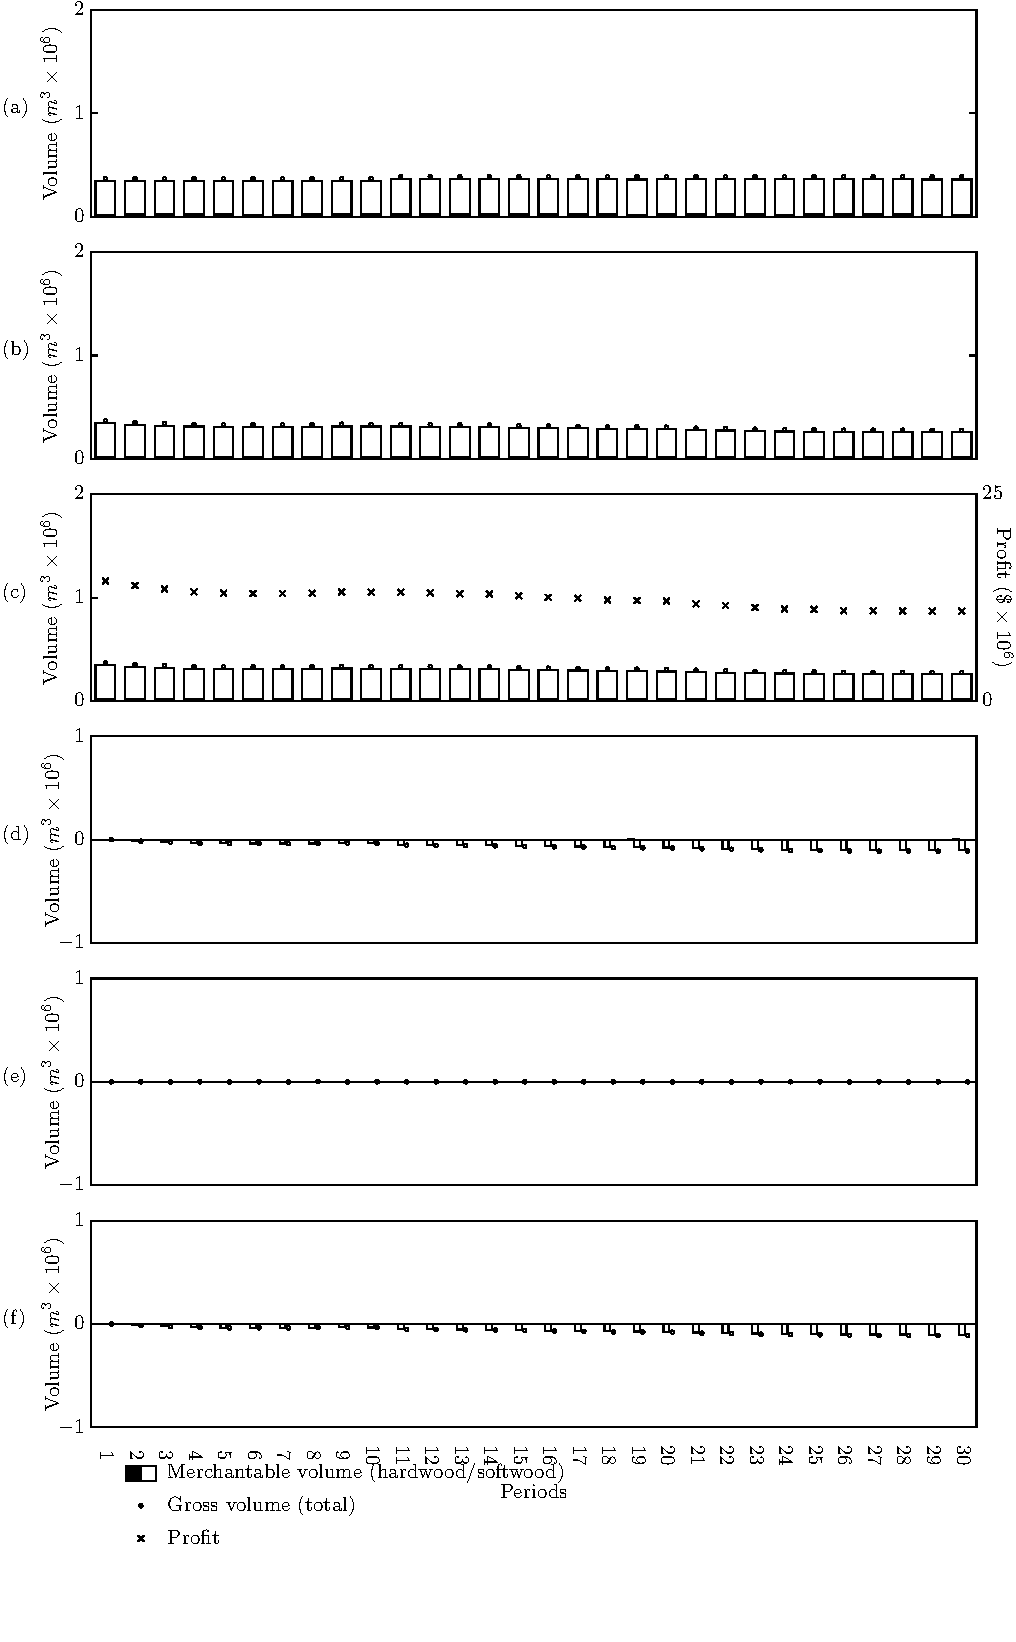
\includegraphics[width=10cm]{images/appendix/s6-1_p30a05}
  \caption{Scenario 6-1\_p30a05 (principal: 30 periods, agent: 5 periods).}
  \label{fig:s6-1_p30a05}
\end{figure}

\begin{figure}[h]
  \centering
  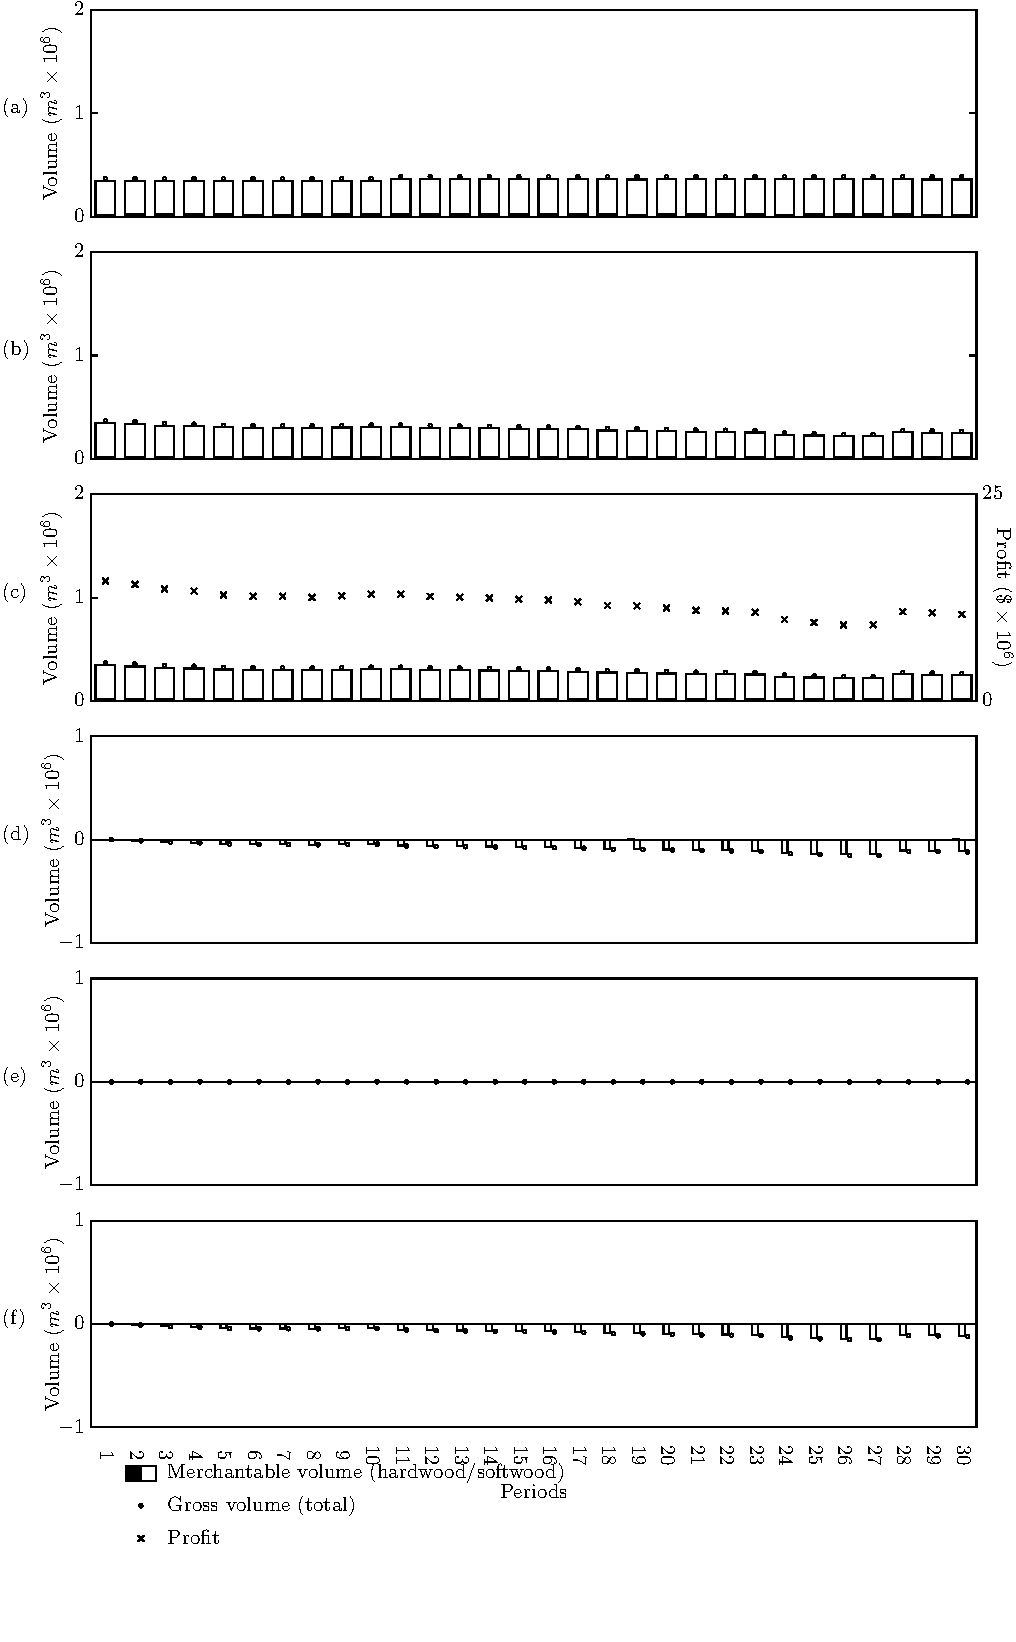
\includegraphics[width=10cm]{images/appendix/s6-1_p30a01}
  \caption{Scenario 6-1\_p30a01 (principal: 30 periods, agent: 1 period).}
  \label{fig:s6-1_p30a01}
\end{figure}


\begin{figure}[h]
  \centering
  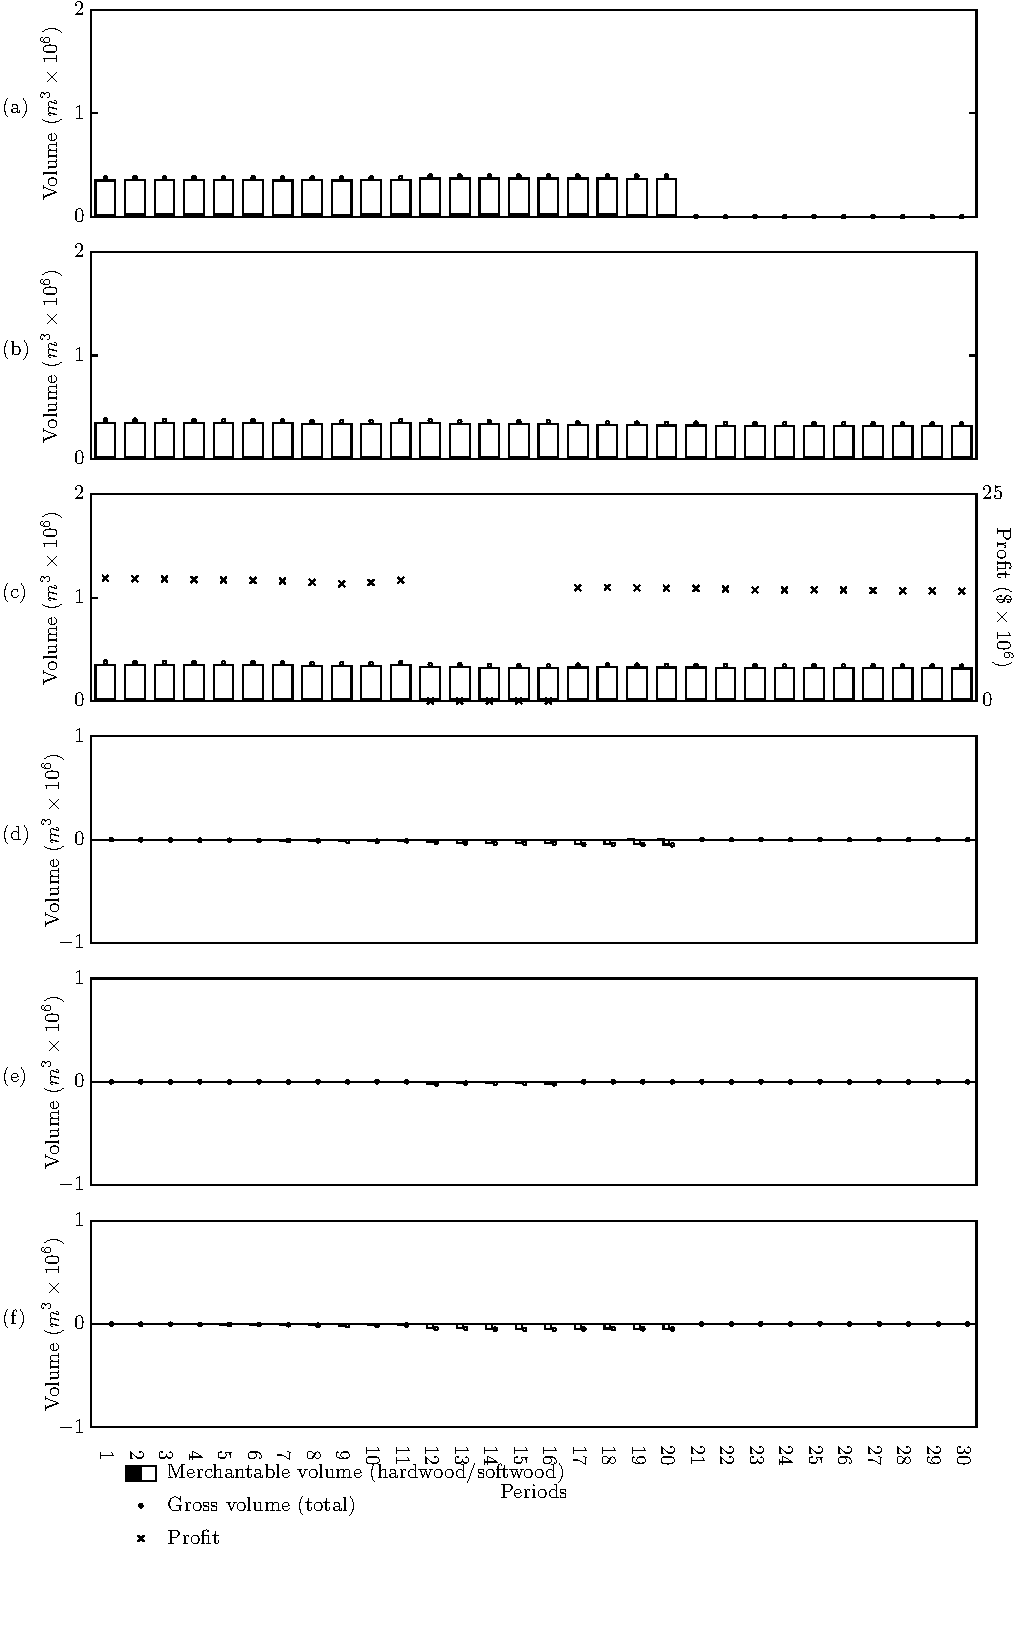
\includegraphics[width=10cm]{images/appendix/s6-1_p20a20}
  \caption{Scenario 6-1\_p20a20 (principal: 20 periods, agent: 20 periods).}
  \label{fig:s6-1_p20a20}
\end{figure}

\begin{figure}[h]
  \centering
  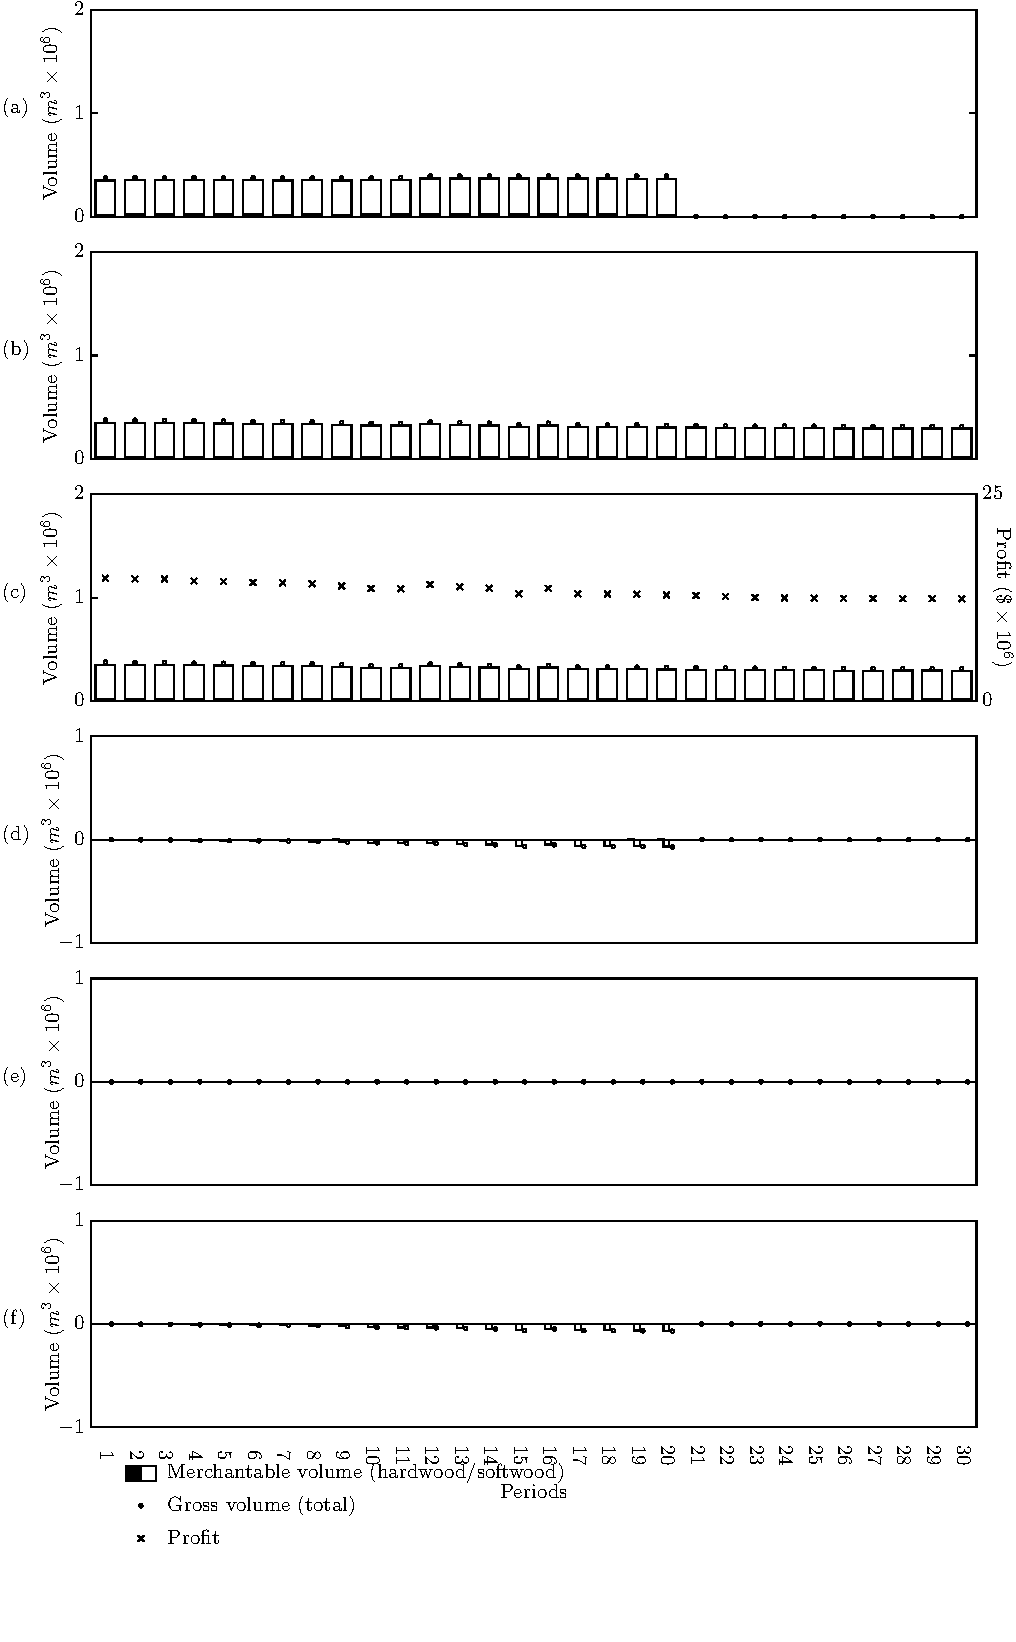
\includegraphics[width=10cm]{images/appendix/s6-1_p20a10}
  \caption{Scenario 6-1\_p20a10 (principal: 20 periods, agent: 10 periods).}
  \label{fig:s6-1_p20a10}
\end{figure}

\begin{figure}[h]
  \centering
  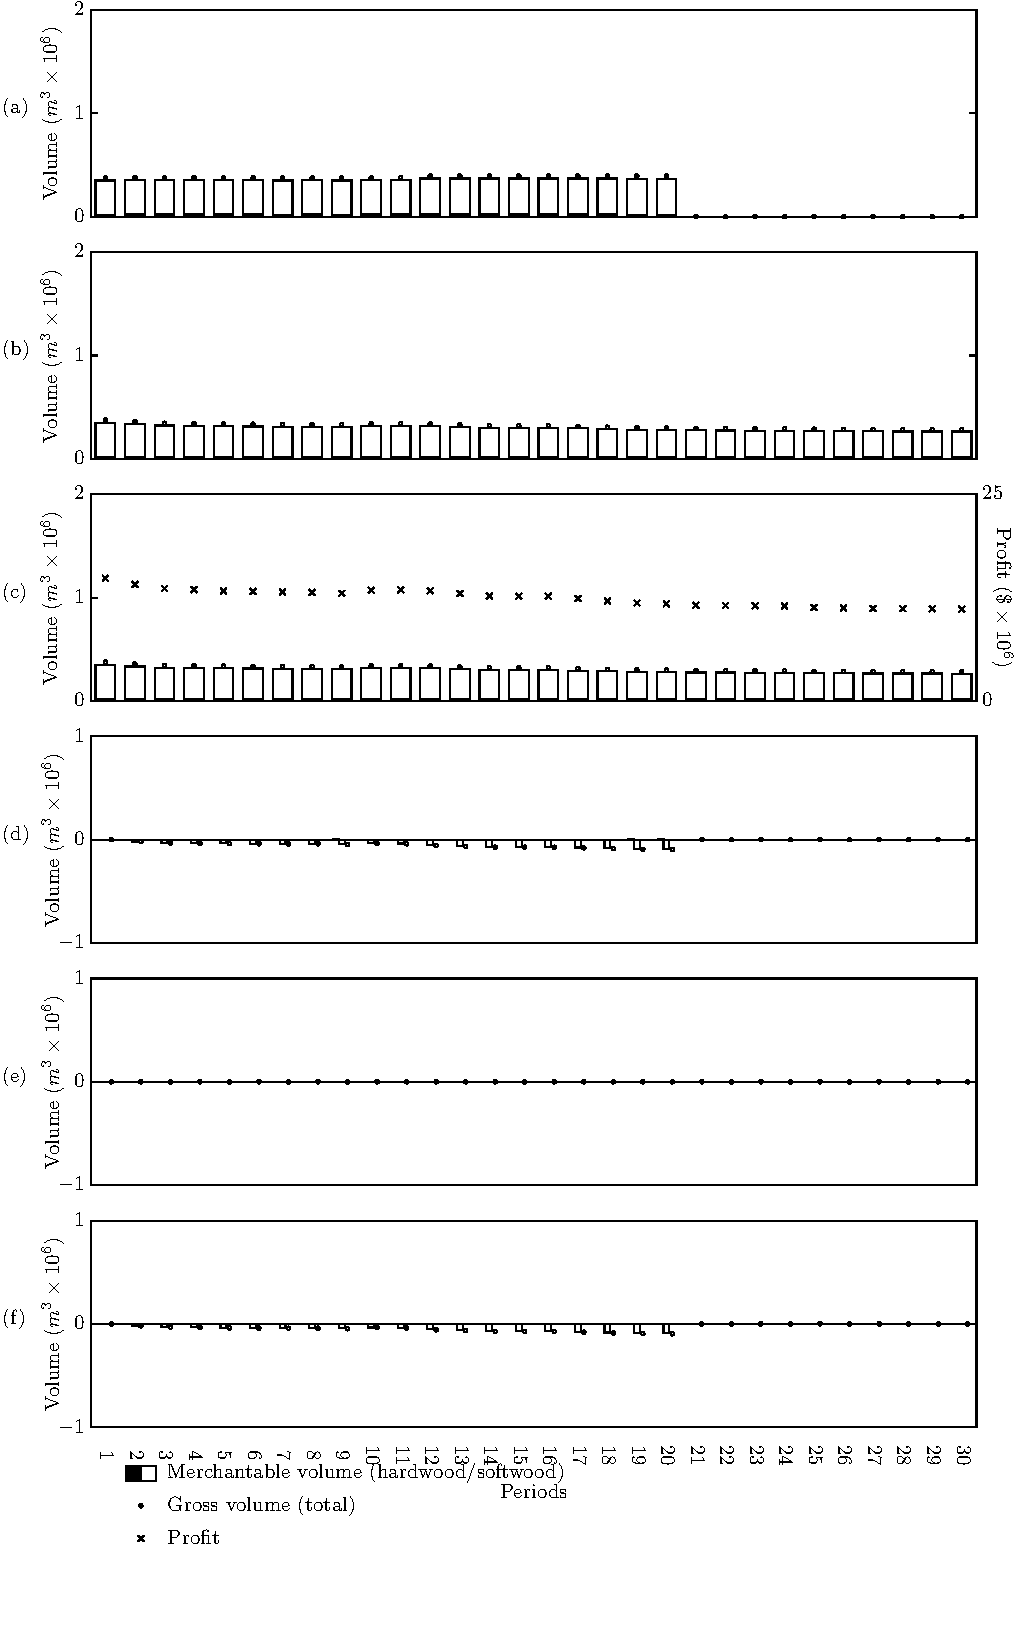
\includegraphics[width=10cm]{images/appendix/s6-1_p20a05}
  \caption{Scenario 6-1\_p20a05 (principal: 20 periods, agent: 5 periods).}
  \label{fig:s6-1_p20a05}
\end{figure}

\begin{figure}[h]
  \centering
  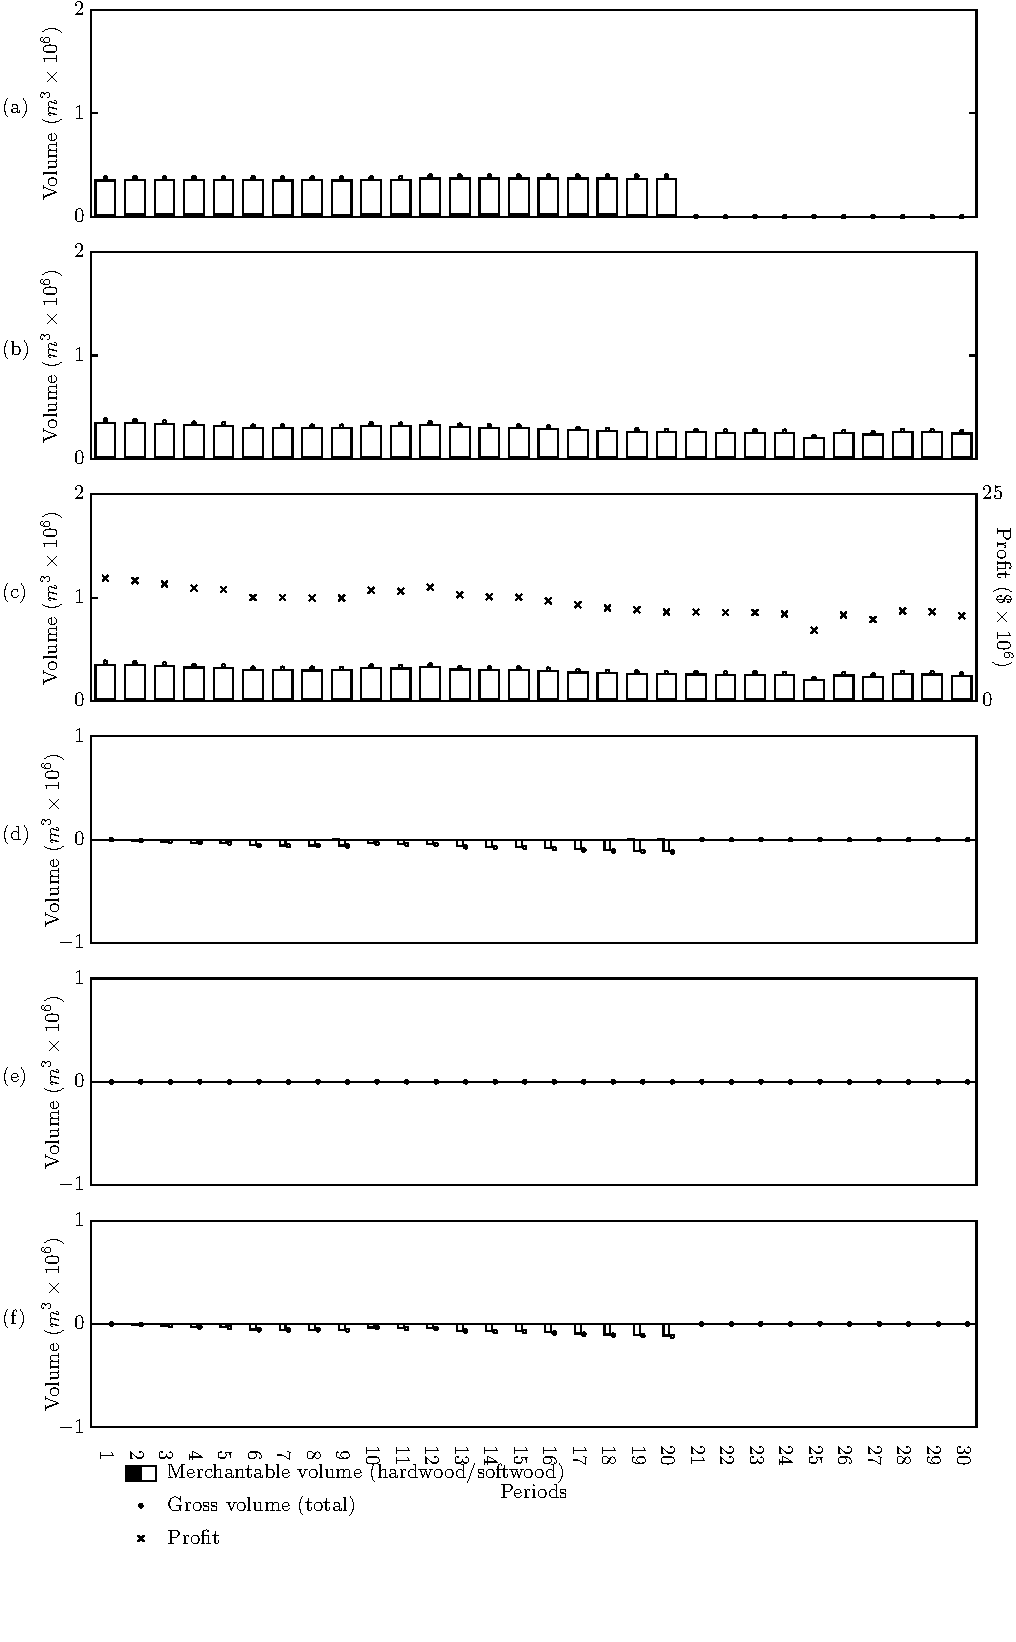
\includegraphics[width=10cm]{images/appendix/s6-1_p20a01}
  \caption{Scenario 6-1\_p20a01 (principal: 20 periods, agent: 1 period).}
  \label{fig:s6-1_p20a01}
\end{figure}


\begin{figure}[h]
  \centering
  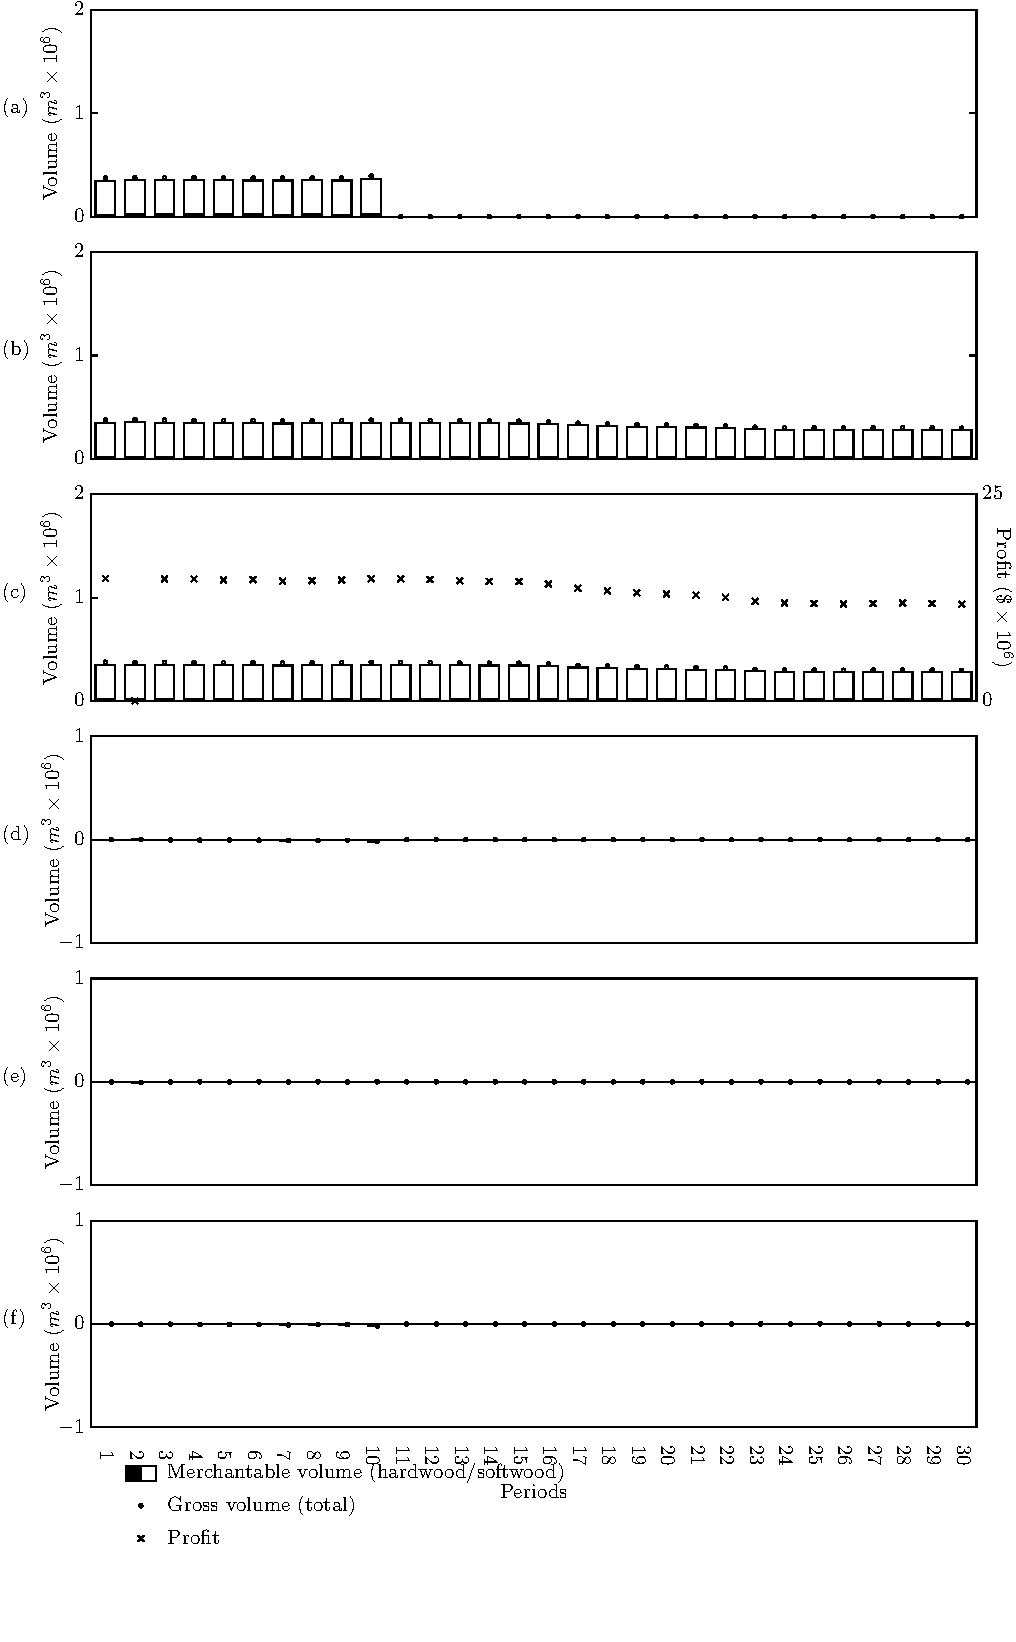
\includegraphics[width=10cm]{images/appendix/s6-1_p10a10}
  \caption{Scenario 6-1\_p10a10 (principal: 10 periods, agent: 10 periods).}
  \label{fig:s6-1_p10a10}
\end{figure}

\begin{figure}[h]
  \centering
  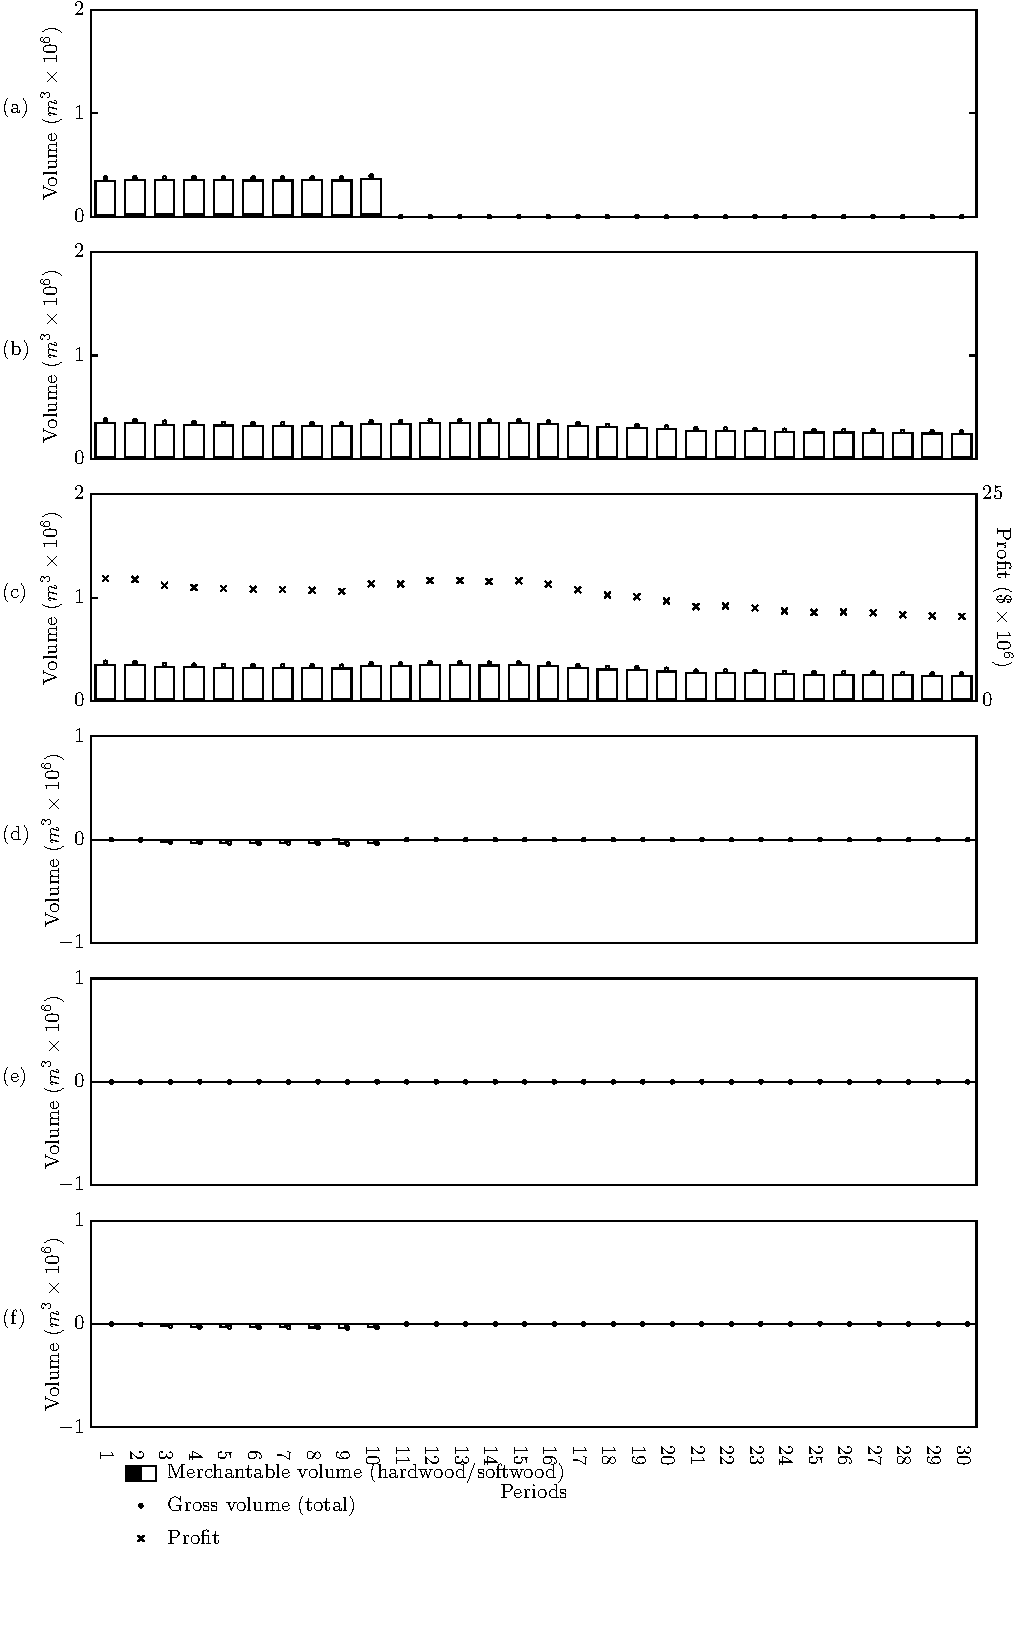
\includegraphics[width=10cm]{images/appendix/s6-1_p10a05}
  \caption{Scenario 6-1\_p10a05 (principal: 10 periods, agent: 5 periods).}
  \label{fig:s6-1_p10a05}
\end{figure}

\begin{figure}[h]
  \centering
  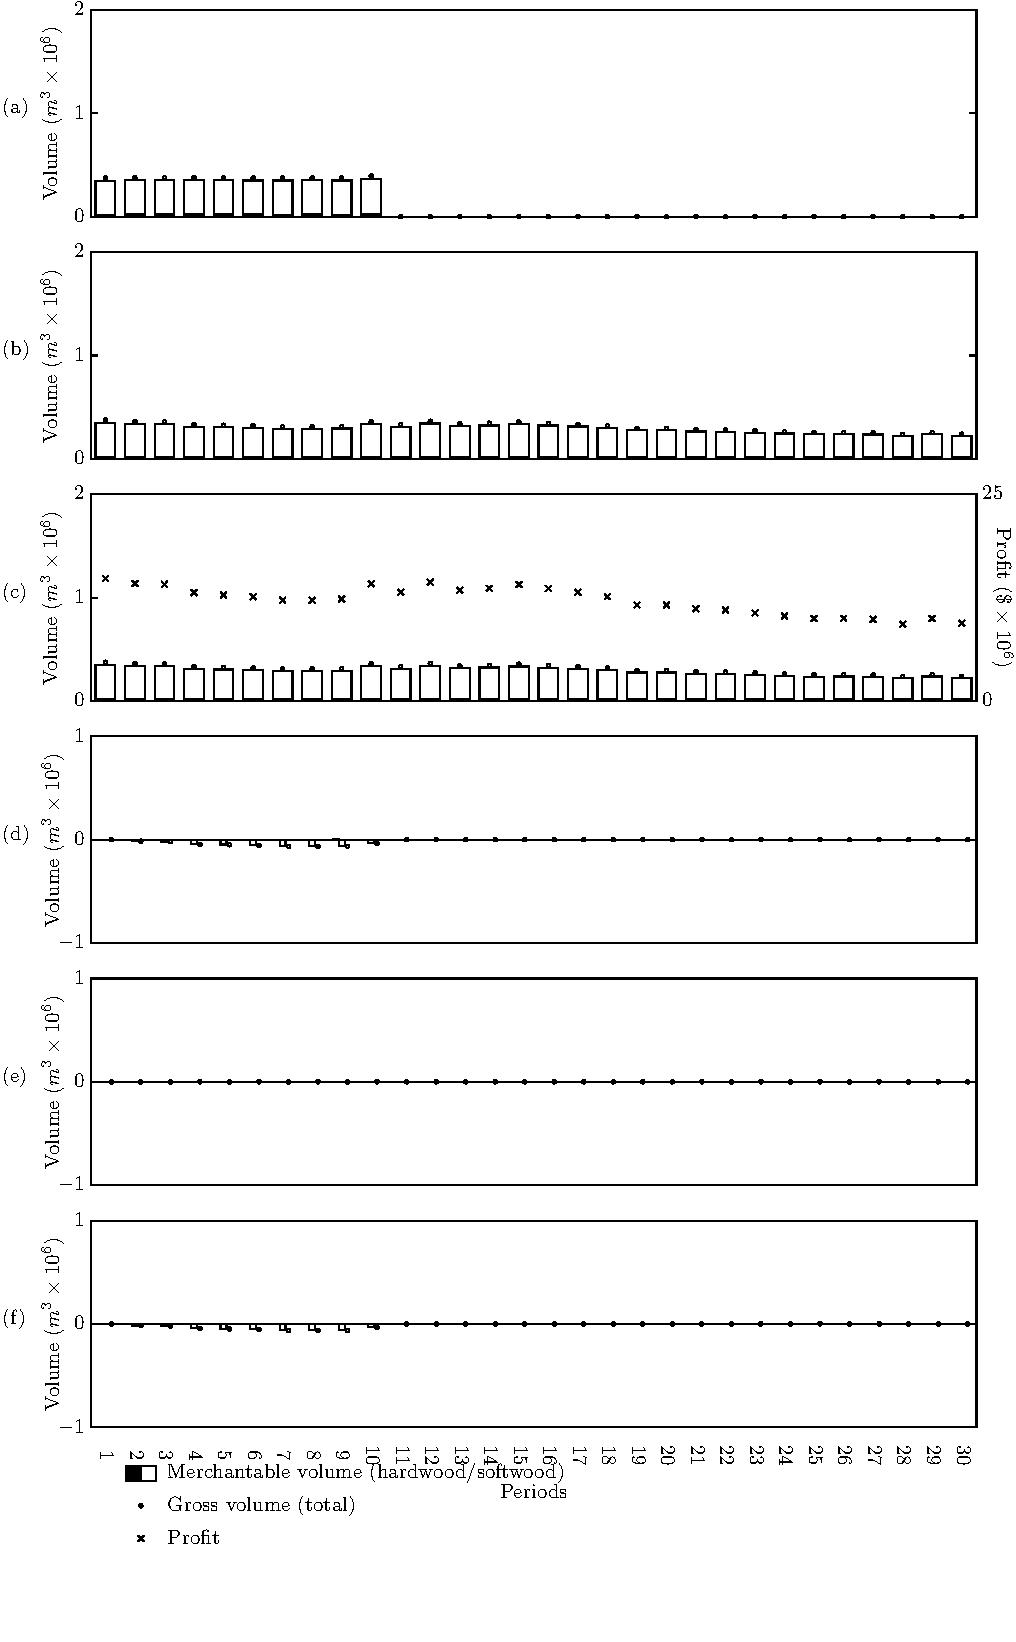
\includegraphics[width=10cm]{images/appendix/s6-1_p10a01}
  \caption{Scenario 6-1\_p10a01 (principal: 10 periods, agent: 1 period).}
  \label{fig:s6-1_p10a01}
\end{figure}


\begin{figure}[h]
  \centering
  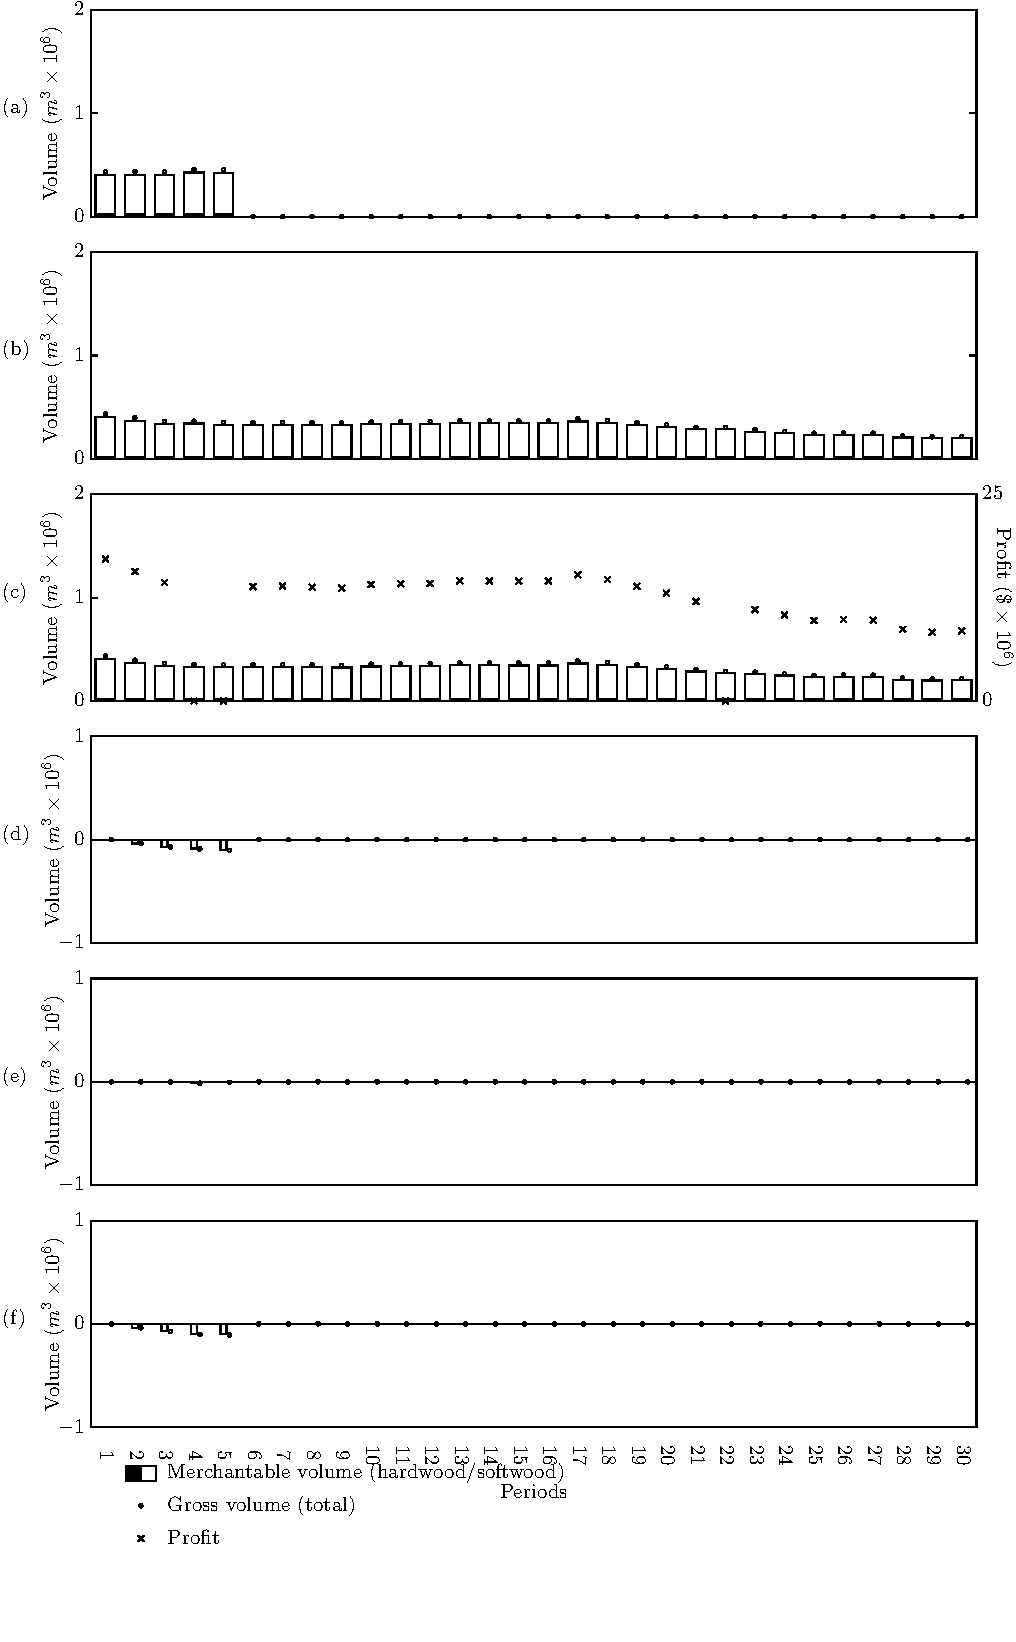
\includegraphics[width=10cm]{images/appendix/s6-1_p05a05}
  \caption{Scenario 6-1\_p05a05 (principal: 05 periods, agent: 5 periods).}
  \label{fig:s6-1_p05a05}
\end{figure}

\begin{figure}[h]
  \centering
  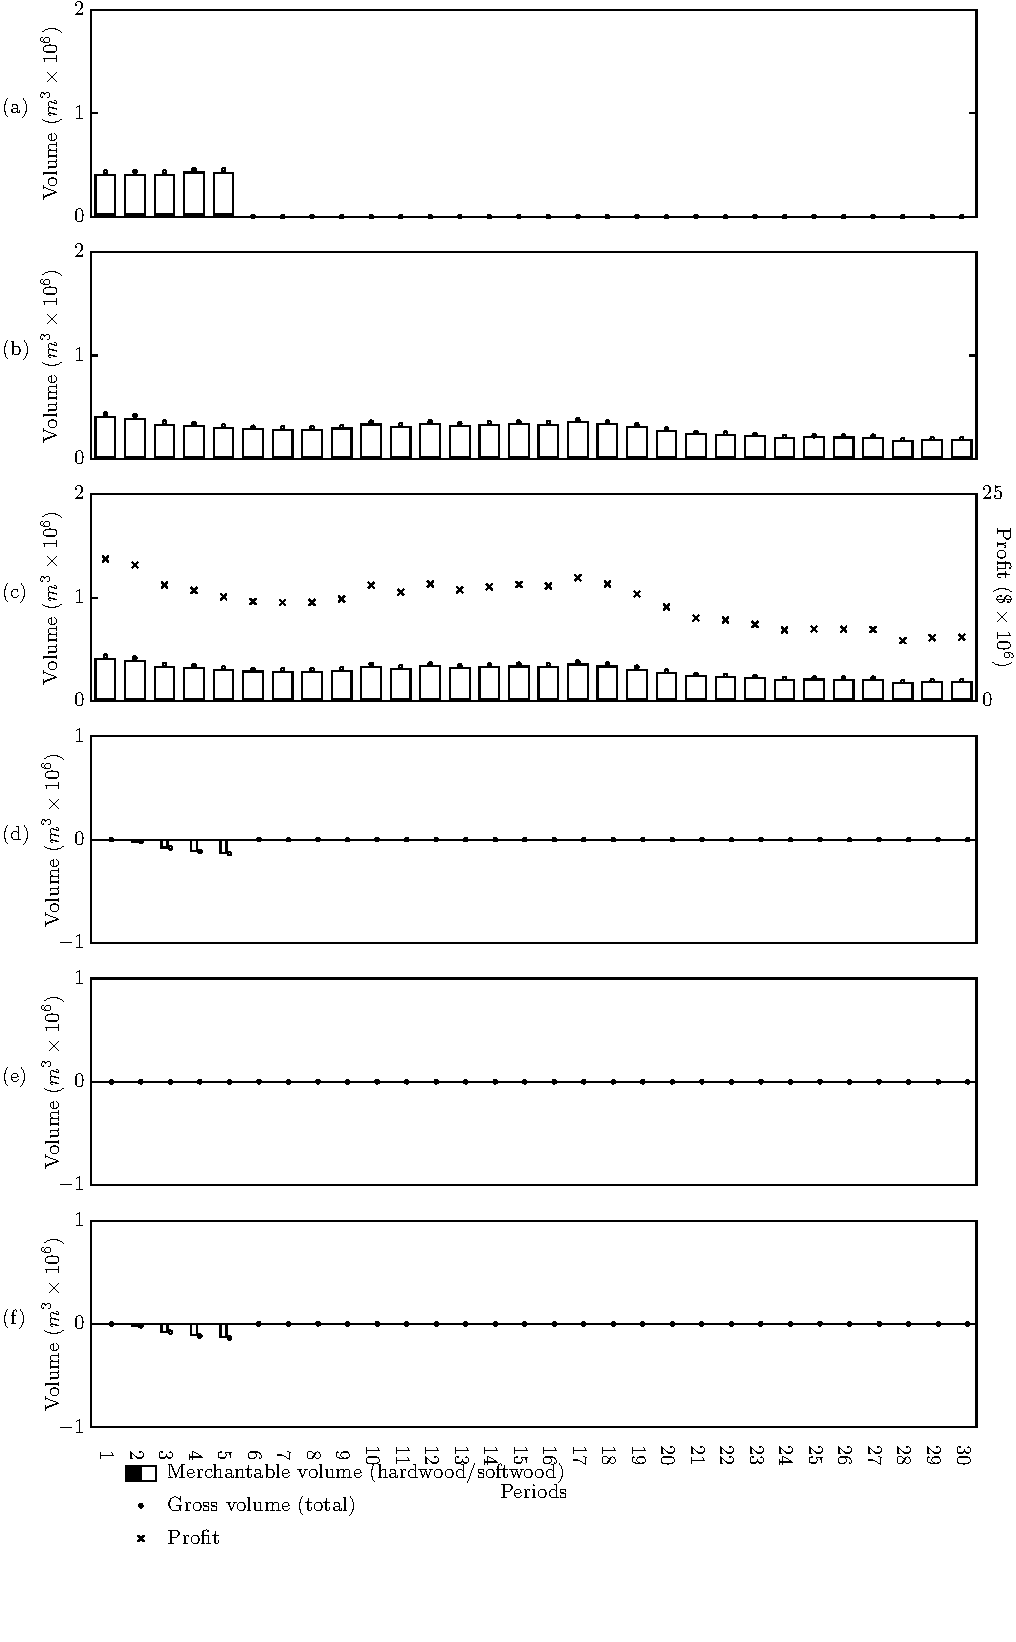
\includegraphics[width=10cm]{images/appendix/s6-1_p05a01}
  \caption{Scenario 6-1\_p05a01 (principal: 05 periods, agent: 1 period).}
  \label{fig:s6-1_p05a01}
\end{figure}


\begin{figure}[h]
  \centering
  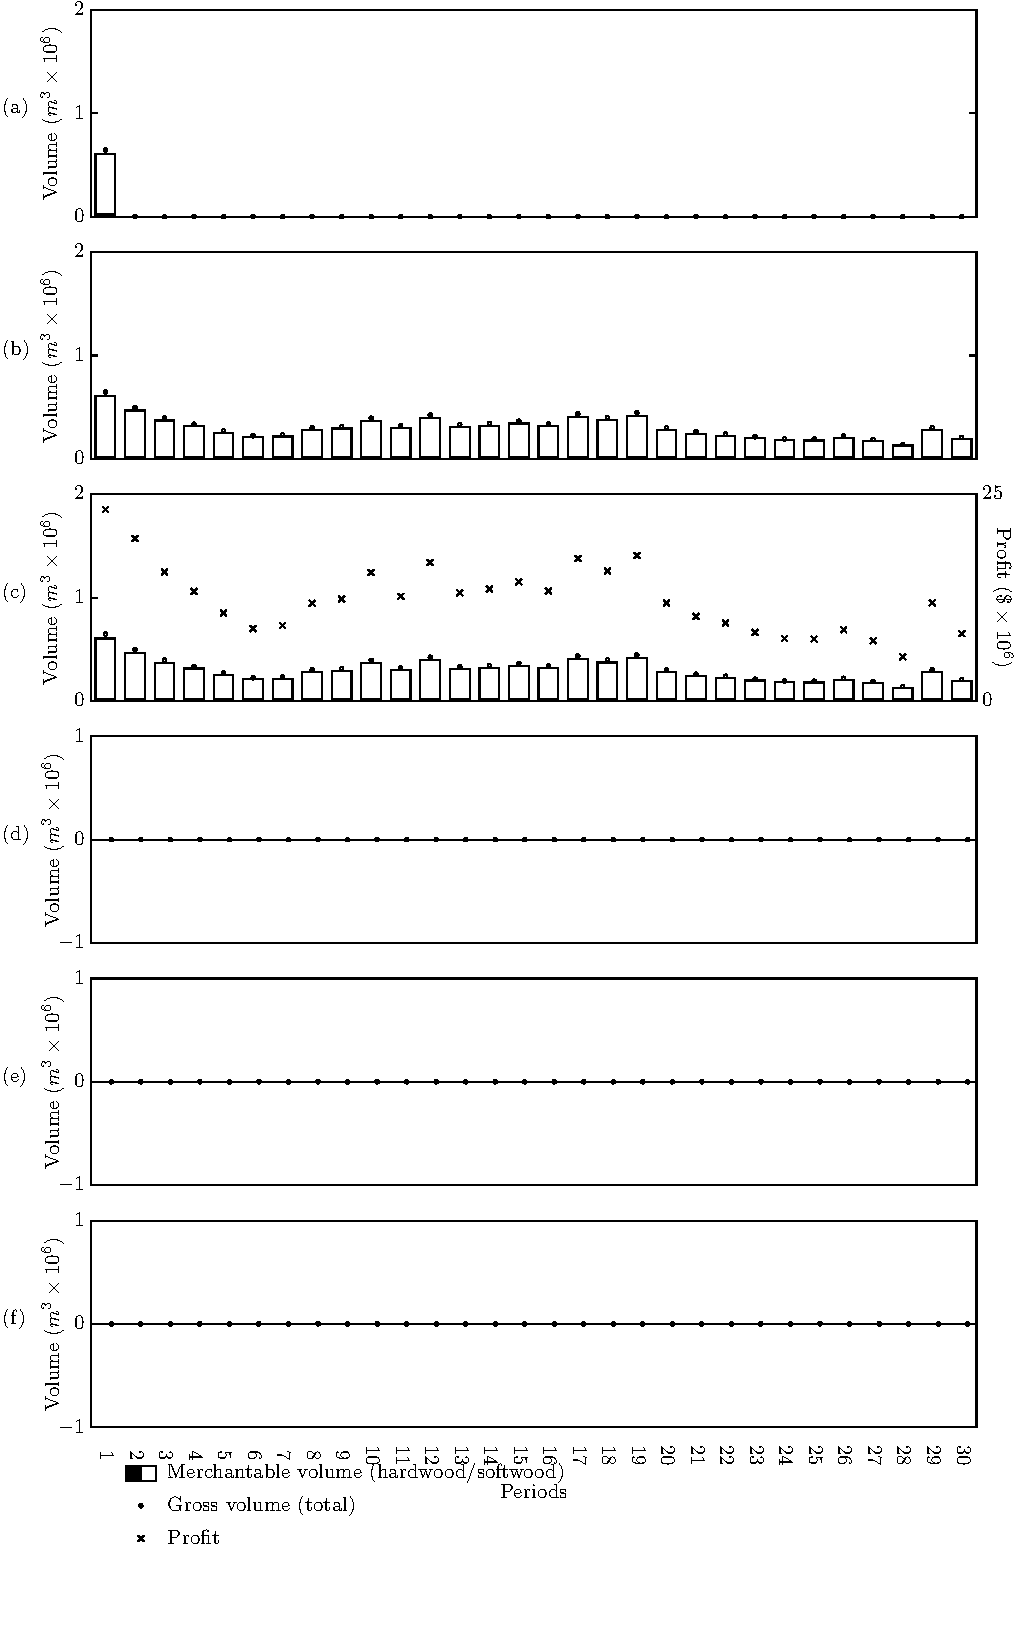
\includegraphics[width=10cm]{images/appendix/s6-1_p01a01}
  \caption{Scenario 6-1\_p01a01 (principal: 1 period, agent: 1 period).}
  \label{fig:s6-1_p01a01}
\end{figure}
